\documentclass[lang=cn,a4paper,newtx]{elegantpaper}

\title{使用经典龙格-库塔法求解波的机械能问题}
\author{姓名:刘畅 \and 学号:202103150815 \and 班级:计算机科学与技术03}

\date{\today}


\usepackage{array}
\usepackage{extarrows}
\usepackage{graphicx}
\usepackage{listings}
\usepackage{geometry}
\usepackage{tabularx}
\newcommand{\ccr}[1]{\makecell{{\color{#1}\rule{1cm}{1cm}}}}
\addbibresource[location=local]{reference.bib} 

\begin{document}

\maketitle

\begin{abstract}
本文介绍了使用四阶龙格-库塔法求解波的机械能问题的方法,
文章将会给出龙格-库塔法(Runge-Kutta methods)的构造原理以及其公式,并用该公式,计算出
某个机械波在二维平面内,在波传播的某时刻,截取介质一部分长度并求出截取段波的机械能。
\keywords{龙格-库塔法,机械能,机械波,介质性质}
\end{abstract}

\section{龙格-库塔法概述}
  \subsection{算法构成原理}
  已知一个微分方程:
  \begin{equation}
    \left\{
    \begin{array}{ll}
      \frac{dy}{dx} &=f(x,y),x\in[a,b]\\
      y(a) &= y_0 
    \end{array}
    \right.
  \end{equation}

  由微分中值定理可知:
  \begin{equation}
      y(x_{i+1})-y(x_i)=y'(\zeta)(x_{i+1}-x_i), \zeta \in (x_i,x_{i+1})
  \end{equation}

  上述(1),(2)式子联立可得:
  \begin{equation}
    y(x_{i+1})=y(x_i)+hf(\zeta,y(\zeta))
  \end{equation}

  其中,$h=x_{i+1}-x_i$为步长,而$f(\zeta,y(\zeta))$为函数$f(x,y)$在区间$[x_i,x_{i+1}]$
  上的平均变化率。我们将$f(\zeta,y(\zeta))$记作$K^*$,那么$K^*$就是曲线$y=f(x)$在区间$[x_i,x_{i+1}]$
  上的斜率。通过对$K^*$近似值的求解,就可以由(3)式推导出一种计算$y(x_{i+1})$近似值的公式。

  我们首先取左端点$x_i$处的斜率,可以得到:
  \begin{equation}
    f(x_i,y(x_i))\approx f(x_i,y_i)\xlongequal[]{\text{(记作)}} K_1
  \end{equation}


  根据上式,我们可以获得作为平均斜率$K^*$的近似值:
  \begin{equation}
    \left\{
    \begin{array}{ll}
      y_{i+1} &=y_i+hK_1,\\
      K_1 &=f(x_i,y_i).
    \end{array}
    \right.
  \end{equation}

  然后再计算右端点$x_{i+1}$处的斜率近似值,可以得到:
  \begin{equation}
    f(x_{i+1},y_{i+1})\approx f(x_i+h,y_i+hf(x_i,y_i))\xlongequal[]{\text{(记作)}} K_2
  \end{equation}

  我们将他们斜率近似值的算数平均值作为平均斜率$K^*$的近似值,可以得到:
  \begin{equation}
    \left\{
    \begin{array}{ll}
      y_{i+1} &=y_i+\frac{h}{2}(K_1+K_2),\\
      K_1 &=f(x_i,y_i),\\
      K_2 &=f(x_i+h,y_i+hK_1).
    \end{array}
    \right.
  \end{equation}

  此时,所得到的结果相比于(5)式,精度更高。
  如果以此类推,在区间$[x_i,x_{i+1}]$上取更多点的斜率的近似值,
  用他们的加权平均值作为平均斜率$K^*$的近似值,那么所得到的结果的精度就会更高。
  形如:
  \begin{equation}
    \left\{
    \begin{array}{ll}
      y_{i+1} &=y_i+h(\alpha_1 K_1+\alpha_2K_2+,\cdots,+\alpha_mK_m)\\
      K_1 &=f(x_i,y_i),\\
      K_2&=f(x_i+\lambda_2h,y_i+\mu_{2}h),\\
      &\vdots\\
      K_m&=f(x_i+\lambda_mh,y_i+\mu_{m}h)
    \end{array}
    \right.
  \end{equation}
  上述公式中,$0\leqslant \lambda_j \geqslant 1$,$y_i+\mu_jh$是$y(x_i+\lambda _jh)$的
  预估值。形如(7)式的运算公式就被称为龙格-库塔公式,简称R-K公式。  
  
  \subsection{经典龙格-库塔法}
  与1.1构成原理所提到的计算方法类似的,通过推导可以得出较为高阶的R-K公式。在众多的R-K公式中
  较为重要的公式就是\textbf{经典R-K公式},形式如下:

  \begin{equation}
    \left\{
      \begin{array}{ll}
        y_{i+1} &=y_i+\frac{h}{6}(K_1+2K_2+2K_3+K_4),\\
        K_1 &=f(x_i,y_i),\\
        K_2 &=f(x_i+\frac{1}{2}h,y_i+\frac{1}{2}K_1),\\
        K_3 &=f(x_i+\frac{1}{2}h,y_i+\frac{1}{2}K_2),\\
        K_4 &=f(x_i+h,y_i+hK_3).
      \end{array}
    \right.
  \end{equation}
  可以开到,经典R-K法实际上是四阶的方法。在解决实际问题时,常常使用的
  就是这种方法。

  相比与欧拉方法(Euler Method),和改进欧拉方法(Improved Euler Method),
  R-K法在结果上的误差要小很多\footnote[1]{参见《数值计算与方法》第四版.朱建新.李友法.的P163例题3结果}
  。不过从计算量方面来看,R-K法的计算量是欧拉法的四倍,是改进欧拉法的两倍。
  所以为了能获得更高的效率,使用经典R-K法时可以将步长选取较大一些。因此在解决同一
  初值问题时,总计算量相当时,R-K法的精度要高于欧拉法和改进欧拉法。

  在这里给出经典龙格-库塔法的代码实现:
  \begin{lstlisting}[language=java]
    public double R_Kmethod(double x, double y, double h)  //classic R-K method
    {
      double k1 = function(x, y);
      double k2 = function(x + h/2, y + h/2 * k1);
      double k3 = function(x + h/2, y + h/2 * k2);
      double k4 = function(x + h, y + h * k3);
      return y + h * (k1 + 2*k2 + 2*k3 + k4) / 6;
    }
  \end{lstlisting}
  需要注意的是,这里给出的代码是异步版本,每次迭代所计算出是当前$y_i$的下一个点$y_{i+1}$的值,而不是
  当前$x_i$的对应值。
  
  \subsection{步长的选择}
  在使用R-K法时,步长的选择是一个很重要的问题。步长太大,会导致误差过大,步长太小,会导致计算量过大,效率太低。
  本次需要解决的是以时间$t$作为自变量的问题,因为理想机械波传播时周期和波长都不变,可以选用固定步长的方法,
  这样无需增加额外的计算量来获得每次迭代的步长。但在实际问题解决时,步长的选择可以使用
  自适应步长的方法。这里介绍一种自适应步长的方法,\textbf{理查森外推法}(Richardson Extrapolation)。

  我们先从节点$x_i$出发,先以$h$为步长,求出$y(x_{i+1})$的一个近似值
  $y_{i+1}^{(h)}$。在$p$阶的方法下,可得:
  \begin{equation}
    y(x_{i+1})-y_{i+1}^{(h)}=ch^{p+1}+O(h^{p+2})
  \end{equation}
  一般情况下,式中系数$c$既依赖于$h$,又依赖于$x_i$。不过,在$h$较小
  的时候,可以近似看为常数。

  然后再以$\frac{h}{2}$为步长,仍从$x_i$出发,经两步计算求得$y(x_{i+1})$的
  另一个近似值$y_{i+1}^{(\frac{h}{2})}$,其中每一步的截断误差约为
  $c(\frac{h}{2})^{p+1}$,则有:
  \begin{equation}
    y(x_{i+1})-y_{i+1}^{(\frac{h}{2})}=2c(\frac{h}{2})^{p+1}+O(h^{p+2})
  \end{equation}
  对(11)式两边同时乘以$2^p$,再减去(10)式,可得:

  \begin{equation}
    y_{i+1}^{(\frac{h}{2})}=\frac{2^py_{i+1}^{(h)}-y_{i+1}^{(\frac{h}{2})}}{2^p-1}+O(h^{p+2})
  \end{equation}
  取$ y(x+i+1)$的近似值$y_{i+1}$,可以转化为:
  \begin{equation}
    y_{i+1}=y_{i+1}^{(\frac{h}{2})}+\frac{1}{2^p-1}(y_{i+1}^{(\frac{h}{2})}-y_{i+1}^{(h)})
  \end{equation}
由$y(x_{i+1}) \approx y_{i+1}$,可得:

\begin{equation}
  y(x_{i+1})-y_{i+1}^{(\frac{h}{2})}\approx \frac{1}{2^p-1}(y_{i+1}^{(\frac{h}{2})}-y_{i+1}^{(h)})
\end{equation}
至此可得,如果将$y_{i+1}^{(\frac{h}{2})}$作为$y(x_{i+1})$的近似值,其误差就可以表示出来:
  \begin{equation}
    \Delta = |y_{i+1}^{(\frac{h}{2})}-y_{i+1}^{(h)}|    
  \end{equation}
使用该误差值判断步长是否恰当,具体方法如下:
  \begin{enumerate}
    \item 若$\Delta \geqslant \varepsilon$($\varepsilon$由精度要求确定),
    则反复将步长折半计算,直到$\Delta <\varepsilon$,并取最后一次步长作为$y_{i+1}$;
    \item 若$\Delta < \varepsilon$,则反复将步长进行加倍计算,直到$\Delta \geqslant \varepsilon$,
    并取上一次步长所得值作为$y_{i+1}$。
  \end{enumerate}


\section{机械波能量与所在传导介质截取长度关系的推导}
  设定理想机械波沿$x$轴正方向传播,其波动方程为:
  \begin{equation}
    y=A \cos \omega(t-\frac{x}{u})
  \end{equation}

  \subsection{波的机械能与能量密度的获取}
    
  波的机械能可以分为两个部分:动能和弹性势能。分别对两个部分与介质体积的关系进行分析。
   \subsubsection{动能部分}
    设介质密度为$\rho$,质量为$m$,体积为$V$,横截面积为$S$,不难得到:
    \begin{equation}
      \begin{aligned}
        dm&=\rho dV\\
        &=\rho S dx\\
      \end{aligned}
    \end{equation}
    根据波动方程可以知道,某质元在$t$时刻的振动速度为:
    \begin{equation}
      v=\frac{\partial y}{\partial t}=-\omega A \sin \omega(t-\frac{x}{u})
    \end{equation}
    那么此时其振动动能为:
    \begin{equation}
      dE_k=\frac{1}{2}(dm)v^2=\frac{1}{2}\rho A^2 \omega^2 \sin^2 \omega(t-\frac{x}{u})Sdx
    \end{equation}

    \subsubsection{弹性势能部分}
    对于介质元而言,其质元弹性势能并不取决于它与平衡点之间的相对距离,而是取决于它和相邻
    质点间的相对位移。如图1所示:
    \begin{figure}[htbp]
      \centering
      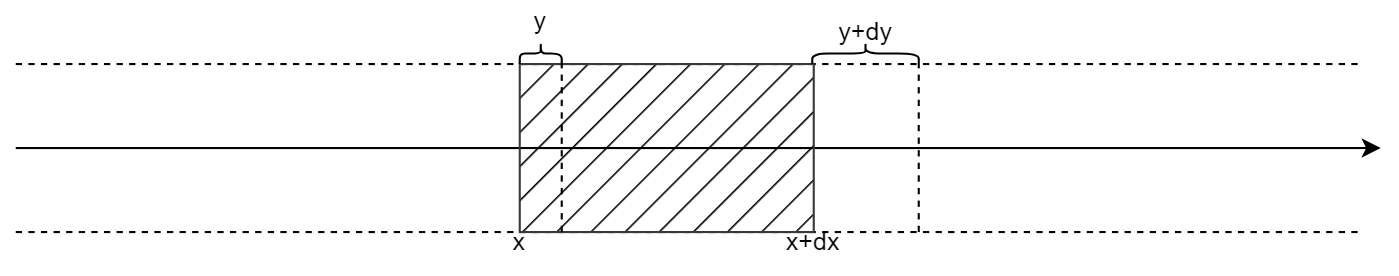
\includegraphics[width=0.9\textwidth]{./image/particleOffset}
      \caption{质元偏移}
    \end{figure}
    可得:
    \begin{equation}
      \frac{\partial y}{\partial x}=\frac{\omega A}{\mu} \sin \omega(t-\frac{x}{u})
    \end{equation}
    设棒的横截面积为$S$,杨氏模量为$E$。杨氏模量的定义式如下:
    \begin{equation}
      E=\frac{F/S}{\partial y/\partial x}
    \end{equation}
    依照该公式获得某质元收到的弹性力:
    \begin{equation}
      F=ES\frac{\partial y}{\partial x}
    \end{equation}
    而已知的弹性力公式形如$F=kdy$,因此可以将弹性力公式和弹簧弹性势能
    公式$dE=\frac{1}{2}k(dy)^2$类比,那么就可以获得质元弹性势能公式:
    \begin{equation}
      \begin{aligned}
      dE_p&=\frac{1}{2}(kdy)dy\\
      &=\frac{1}{2}ES\frac{\partial y}{\partial x}\frac{\partial y}{\partial x}dx\\
      &=\frac{1}{2}ES(\frac{\partial y}{\partial x})^2dx\\
      &=\frac{1}{2}\rho S\omega^2A^2\sin^2\omega(t-\frac{x}{u})dx
      \end{aligned}
    \end{equation}
    至此,就可以根据(19)式和(23)式获得关于波的机械能和介质空间截取长度之间的关系:
    \begin{equation}
      \begin{aligned}
        dE&=dE_k+dE_p\\
        &=\rho SA^2 \omega^2 \sin^2 \omega(t-\frac{x}{u})dx
      \end{aligned}
    \end{equation}

\section{使用经典龙格-库塔法求解波的机械能}
  \subsection{机械能的求解和截取长度与其的关系}
    在上述推导中,获得了波的机械能和介质体积之间的关系(24)式,
  现在对该式子进行转化,可以得到:
  \begin{equation}
    \frac{dE}{dx}= \rho S A^2 \omega^2 \sin^2 \omega(t-\frac{x}{u})
  \end{equation}
  不难看出,如果我们将介质某处的位置$x$看作该方程的唯一自变量,那么这就是一个常微分变量方程,
其应变量就是机械能$E$。

  而对于一个实体介质,在其初始位置$x=0$处,其质量$m=0$,显然其机械能$E=0$。
  因此可以得到一个关于方程初值的一个等式:
  \begin{equation}
    E(0)=0
  \end{equation}
  联立(25)(26)方程,就可以得到一个可以使用经典龙格-库塔法求解的方程:
  \begin{equation}
    \left\{
    \begin{array}{ll}
      \frac{dE}{dx}&= \rho SA^2 \omega^2 \sin^2 \omega(t-\frac{x}{u})\\
      E(0)&=0
    \end{array}  
    \right.
  \end{equation}

  可以观察到,在这个微分方程中实际上有至少2个未知变量。方程参数中,介质密度$\rho$
  ,振幅$A$,角频率$\omega$,波速$u$都是根据波源得到的波本身的特性参数。介质空间位置$x$是这里规定的自变量,
  而时间变量$t$在原关系式(24)中是自变量。但是在求解时,我们
  可以将这个变量看作环境参数,并使用龙格-库塔法求解常微分方程。

  定义这个函数function代码如下:
  \begin{lstlisting}[language=java]
    public double function(double x , double t)
    {
      return rho*S*Math.pow(A,2)*Math.pow(omega,2)*Math.pow(Math.sin(omega*(t-x/u)),2);
    }
  \end{lstlisting}

现在构造各种参数,设圆周率$\pi=3.1415$,角速度$\omega=2\pi$,介质密度$\rho=1.21$,介质
横截面积$S=3.0$,波速$u=10.0$,截断位置从$x_{min}=0$到$x_{max}=40$,
步长为$h=1.0$,时间参数的选择必须满足$u\cdot t \leqslant x_{max}$,这里以$t=4$为例。

为了直观获得波的机械能随截断位置长度的变化,程序在输出$x$,$y$关系表的同时,使用Java语言
的
jfreechart库的元件绘制其对应函数图像。下面给出主函数代码:
\begin{lstlisting}[language=java]
  public static void main(String[] args)
    {

        final double h = 1.0;
        double t = 3;
        double x = 0;
        double y = 0;
        int n =  (int)(max-min)/(int)h;
        XYSeries series = new XYSeries("xySeries");
        System.out.println("x = " + String.format("%.6f",x ) + " y = " + String.format("%.6f",y ));
        for(int i = 0; i <= n; i++)
        {
            y = R_Kmethod(x,y,t,h);
            x += h;
            System.out.println("x = " + String.format("%.6f",x ) + " y = " + String.format("%.6f",y ));
            series.add(x,y);

        }
        XYSeriesCollection dataset = new XYSeriesCollection();
        dataset.addSeries(series);
        JFreeChart chart = ChartFactory.createXYLineChart
                (
                "the relationship between cut-off length and wave wave mechanical energy", // chart title
                "x", // x axis label
                "E", // y axis label
                dataset, // data
                PlotOrientation.VERTICAL,
                false, // include legend
                false, // tooltips
                false // urls
        );

        ChartFrame frame = new ChartFrame("Wave mechanical energy", chart);
        frame.pack();
        frame.setVisible(true);
        frame.setDefaultCloseOperation(JFrame.EXIT_ON_CLOSE);
    }
\end{lstlisting}
以下为样例的部分输出结果($x\in[15,20]$):

\begin{table}[ht]
  \centering
  \begin{tabular}{|c|c|}
  \hline
      $x_i$ & $E_i$ \\ \hline
      15 & 26869.206236 \\ \hline
      16 & 27304.443988 \\ \hline
      17 & 29615.344723 \\ \hline
      18 & 33083.774380 \\ \hline
      19 & 35392.014871 \\ \hline
      20 & 35825.608315 \\ \hline
  \end{tabular}
  \caption{截取长度与机械能部分关系}
\end{table}
以下为输出的关系图:
\begin{figure}[htbp]
  \centering
  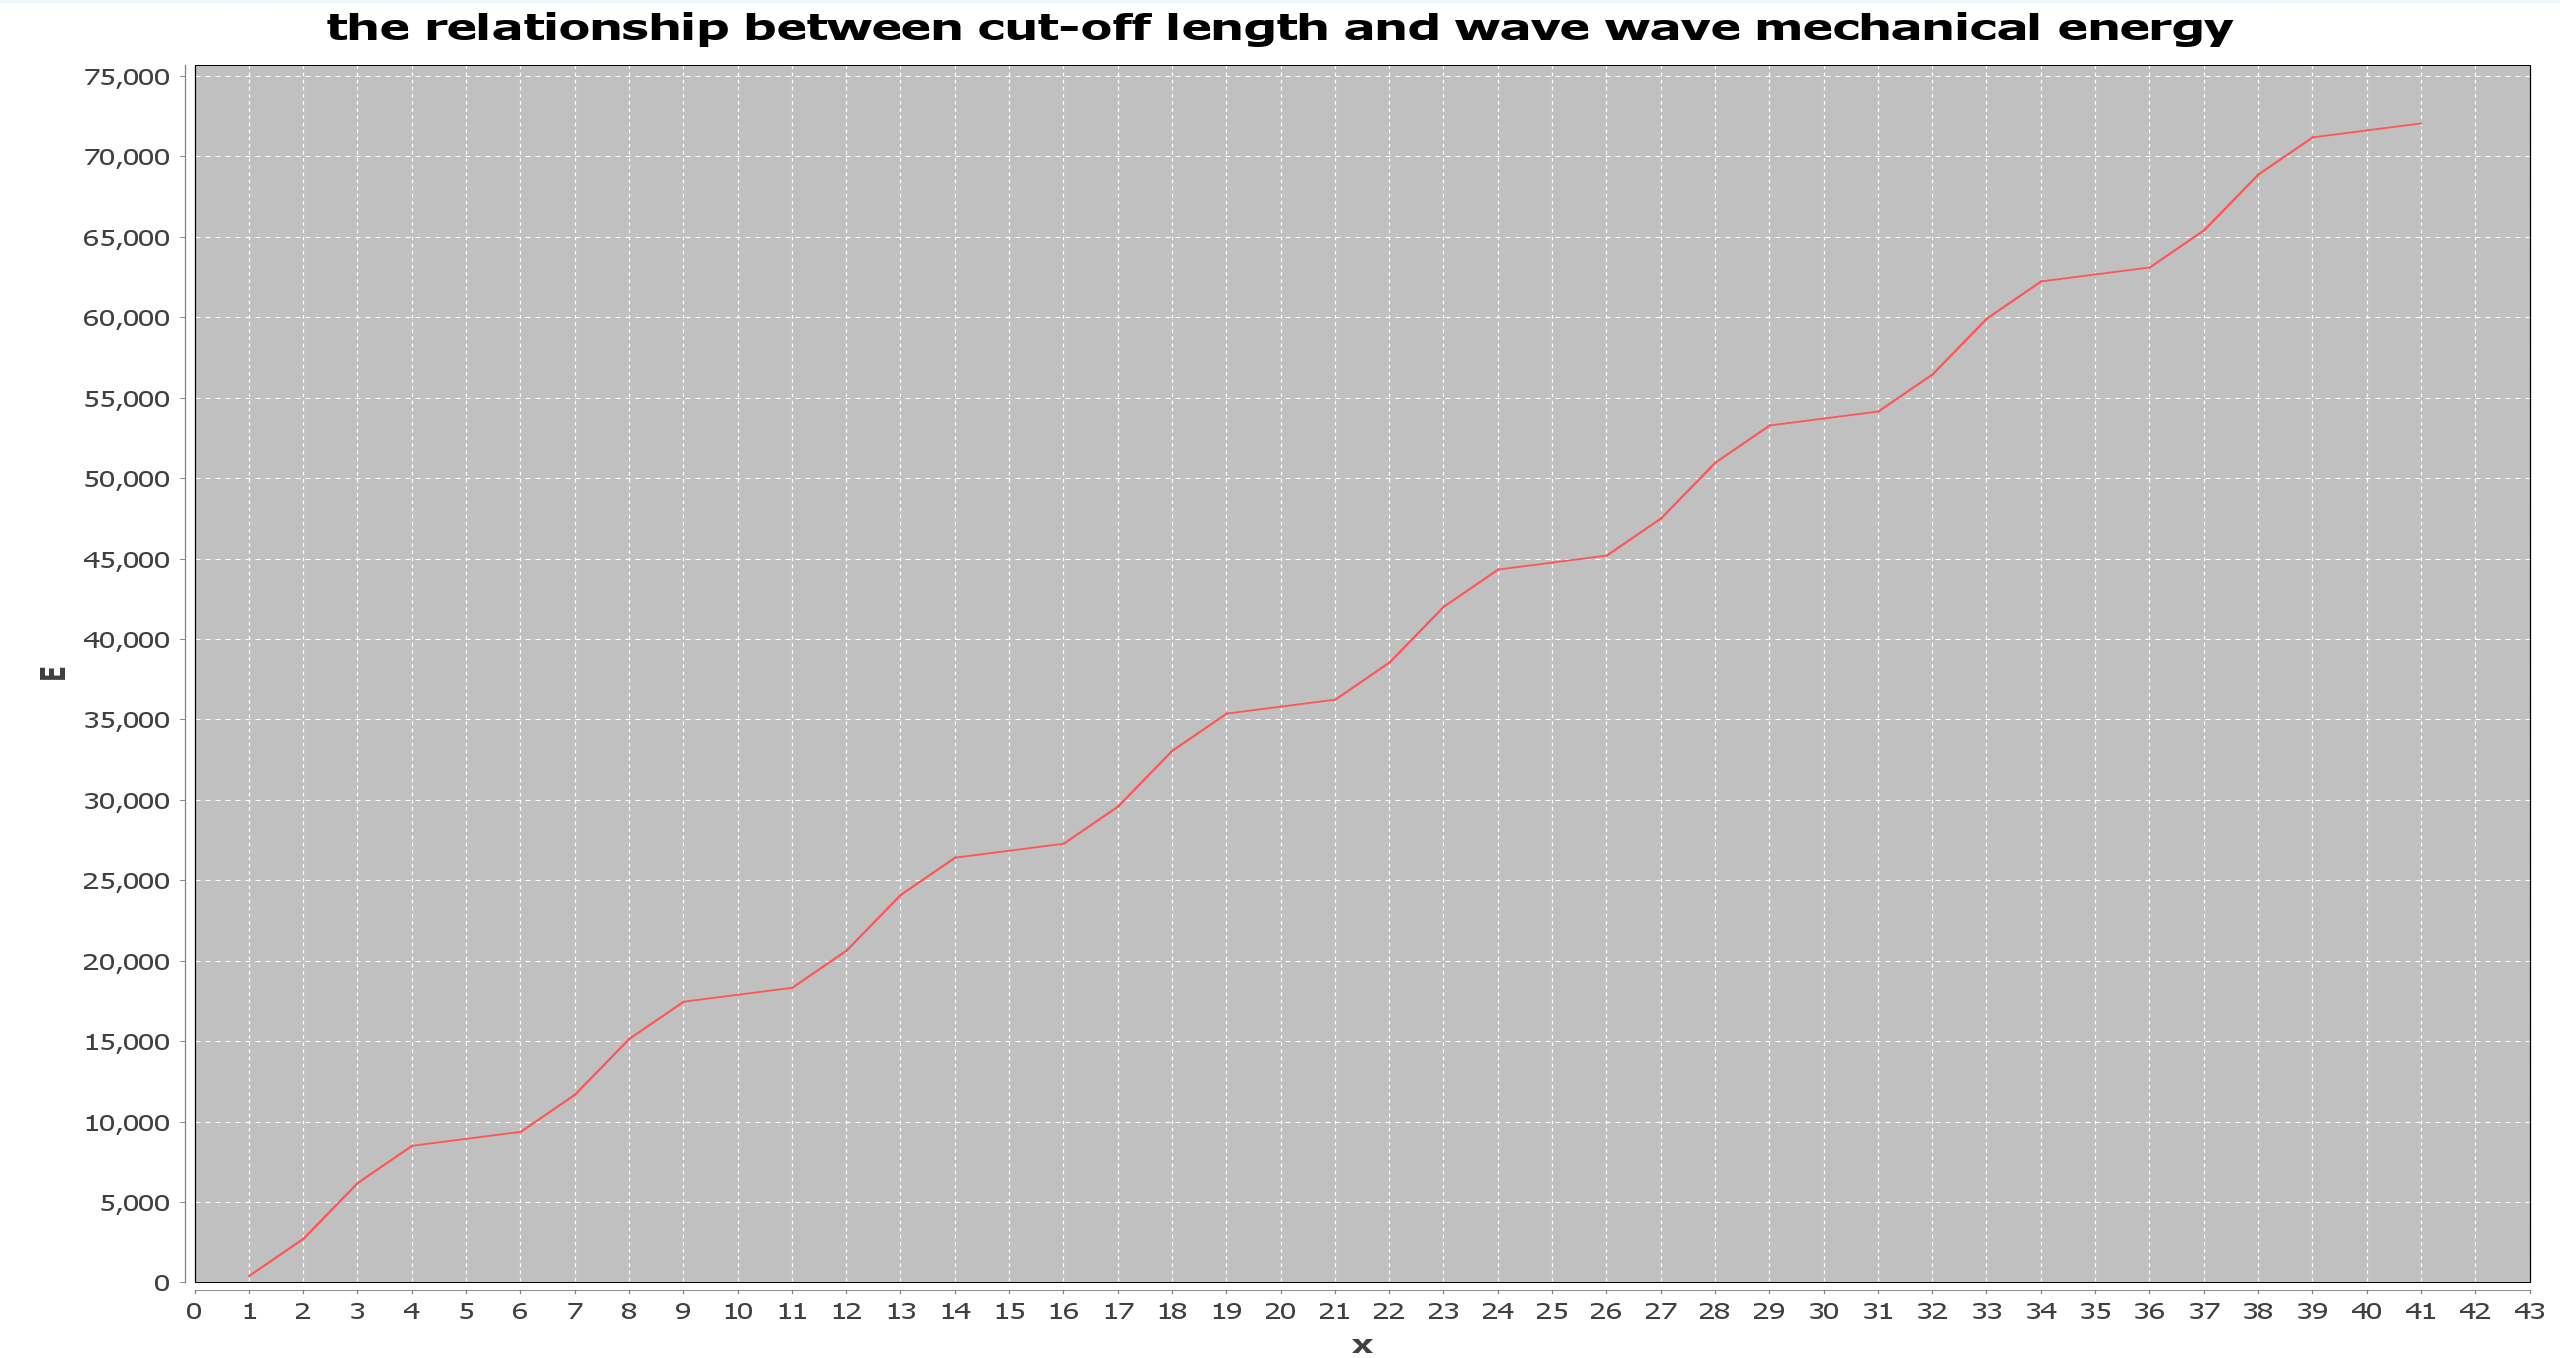
\includegraphics[width=\textwidth]{./image/functionRelationChart}
  \caption{介质空间截取长度与机械能的关系图}
\end{figure}

通过观察输出的数值和函数图像,波的机械能随着截断长度的上升呈周期性波动上升的状态,

 \subsection{求解结果误差估算}
 根据(24)式所给的关系,通过积分将其转化为准确值的计算公式。对于
  截取$x\in[a,b]$,机械能计算公式为:
  \begin{equation}
    E=\frac{1}{2}\rho SA^2 \omega^2\{(b-a)+\frac{u}{2\omega}[\sin 2\omega(t-\frac{b}{u})-\sin 2\omega(t-\frac{a}{u})]\}
  \end{equation}
  依照该公式,使用函数计算出截取长度为$[0,40]$的机械能的准确值,代码如下:
\newpage
  \begin{lstlisting}
    public static double accurate(double a, double b, double t)
    {
        return 0.5*rho * S * Math.pow(A, 2) * Math.pow(omega, 2) * 
        ((b - a) + (u / (2 * omega)) * 
        (Math.sin(2 * omega * (t - (b / u))) - Math.sin(2 * omega * (t - (a / u)))));
    }
  \end{lstlisting}
依照程序运行结果拓展表1,给出部分的误差结果如下:
  \begin{table}[ht]
    \centering
    \begin{tabular}{|c|c|c|c|}
    \hline
        $x_i$ & $E_i$ & $E_{accurate}$ & $|E_i-E_{accurate}|$\\ \hline
        15 & 26869.206236 & 26869.205517 & 0.000720\\ \hline
        16 & 27304.443988 & 27305.673661 & 1.229673\\ \hline
        17 & 29615.344723 & 29616.102857 & 0.758134\\ \hline
        18 & 33083.774380 & 33083.010661 & 0.763719\\ \hline
        19 & 35392.014871 & 35390.782027 & 1.232844\\ \hline
        20 & 35825.608315 & 35825.607355 & 0.000960\\ \hline
    \end{tabular}
    \caption{机械能计算结果与其准确值误差}
  \end{table}

在程序输出的所有结果中,其误差也存在周期性规律。若定义误差大于1的项为“大误差”,否则为“小误差”,那么
自$x=1$项开始,误差呈现按顺序“大小小大小”的周期性规律。猜测是经典R-K法本身性质所导致的。其计算的
相对误差$|e_r^*| \leqslant 0.282\%$,所以可以判断其计算结果是较为准确的。

\section*{总结}
  本文概述了Runge-Kutta方法的概念及其经典四阶版本的形式。并通过基本物理方程推导出
  平面波在介质中传播时的机械能与截取长度的微分方程式。利用经典R-K法对机械能进行求解,并获得了
  截取长度和机械能的关系式,分析了该计算方法的大概误差特征。

  数值计算方法这门课程所涉及的内容对于程序开发而言拥有重要的价值。在现实中所碰到的计算问题,我们也许可以借助
  自己的知识进行计算,但在很多情况下无法得出准确数值,甚至无法直接计算。对于计算机而言,我们通过非直接的运算
  手段,可以让其获得那些无法计算的数值的近似。这也是数值计算方法的价值之一。而如何让计算机获得更加
  精确的数值,则是数值计算方法的研究方向之一。通过将计算方法用于实际问题的探究过程,我深刻体会到了其
  重要意义。更具体的,我对研究的方法有了更深入的认识。例如本次解决问题时发现的经典R-K法的误差规律,
  并了解到,如果我的取数精确度不高,或者取过小的数字,那么R-K法所得到的误差就有可能被放大。以上便是我
  对这次研究简短的体会。
\nocite{*}
\printbibliography[heading=bibintoc, title=\ebibname]

\appendix
%\appendixpage
\addappheadtotoc

\end{document}
